\documentclass{article}
\usepackage[utf8]{inputenc}

\usepackage{graphicx}
\usepackage{float}
\usepackage{titlesec}
\usepackage[bottom]{footmisc}
\usepackage[italian]{babel}
\usepackage{geometry}
\geometry{a4paper, top=1cm, bottom=3cm, left=3cm, right=3cm,}

\graphicspath{{images/}}

\title{{\huge IoT- Final Project}}
\author{Daniele Antonio Emanuele Carta - 10573704\\Cristian Carmine Spagnuolo - 10745353}

\begin{document}
\maketitle
\section{Introduzione}
Questo elaborato si prefigge come obiettivo la progettazione e l’implementazione di un sistema di monitoraggio che fonda il suo funzionamento su \emph{Node-RED}, un framework per la programmazione flow-based.\\

La soluzione proposta, chiamata di seguito \emph{Node-Cloud}, offre all’utente finale la possibilità di visualizzare le informazioni di contesto raccolte dai sensori connessi e di modificare il funzionamento dei dispositivi stessi. Per rendere il sistema adatto al monitoraggio di ambienti totalmente diversi sono state previste due importanti caratteristiche:
\begin{itemize}
    \item l’assenza di uno schema fisso per la rappresentazione logica dei sensori consente di registrare dispositivi di natura e produttori diversi;
    \item la presenza di un \emph{Context Broker} risolve il problema dell’eterogeneità dei dati raccolti, consentendo alle diverse componenti applicative di accedere alle informazioni in modo indipendentemente dalla loro origine.
\end{itemize}

Nel capitolo successivo sarà presentato il sistema di monitoraggio realizzato, denominato \emph{Node Cloud}. Ne sarà descritta l’architettura generale per poi spostare il focus sulle singole componenti. Inoltre, saranno analizzate le modalità di interazione tra le varie componenti e le funzionalità esibite, le quali sono state individuate a valle di un’analisi del dominio del problema.\\

In conclusione, saranno riportate alcune osservazioni finali sul lavoro svolto, soffermandosi sulle limitazioni dell’attuale implementazione e su eventuali sviluppi futuri.

\section{Node Cloud}
\subsection{Architettura}
Node-Cloud è stato realizzato secondo un’architettura a multi-tier, figura \ref{fig:node-cloud-architecture}. L’idea di fondo di questo modello architetturale è quella di realizzare un’applicazione costituita da una serie di servizi indipendenti, ciascuno dei quali con scope molto specifico e limitato. 
Diversi sono i vantaggi:
\begin{itemize}
    \item \textbf{Manutenibilità:} con la separazione e lo snellimento dei vari tier, operazioni di manu[]tenzione e aggiornamento sono rese più semplici. Ciò rende il sistema più flessibile e in grado di adattarsi ai cambiamenti dell’ambiente in cui è immerso. Inoltre, essendo l’accoppiamento ridotto al minimo, per la sostituzione di una componente è sufficiente che il servizio esponga la medesima interfaccia e implementi gli stessi meccanismi di comunicazione.
    \item \textbf{Scalabilità:} fa riferimento alla possibilità di replicare ogni tier, anche su macchine diverse, per poter rispondere dinamicamente alle esigenze. La replicazione delle componenti, oltre a consentire la possibilità di gestire più richieste contemporaneamente, aumenta anche la tolleranza ai guasti. È tuttavia necessaria l’introduzione di un load balancer per poter distribuire equamente il carico tra le varie repliche.
    \item[] \textbf{Flessibilità del linguaggio di sviluppo:} essendo il sistema costituito da più componenti è possibile scegliere linguaggio di programmazione e framework più adatti a quel servizio. La ridefinizione di un tier o una sua eventuale migrazione di tecnologia non richiederà alcuna modifica alle componenti residue.
\end{itemize}
\begin{figure}[htb]
    \centering
    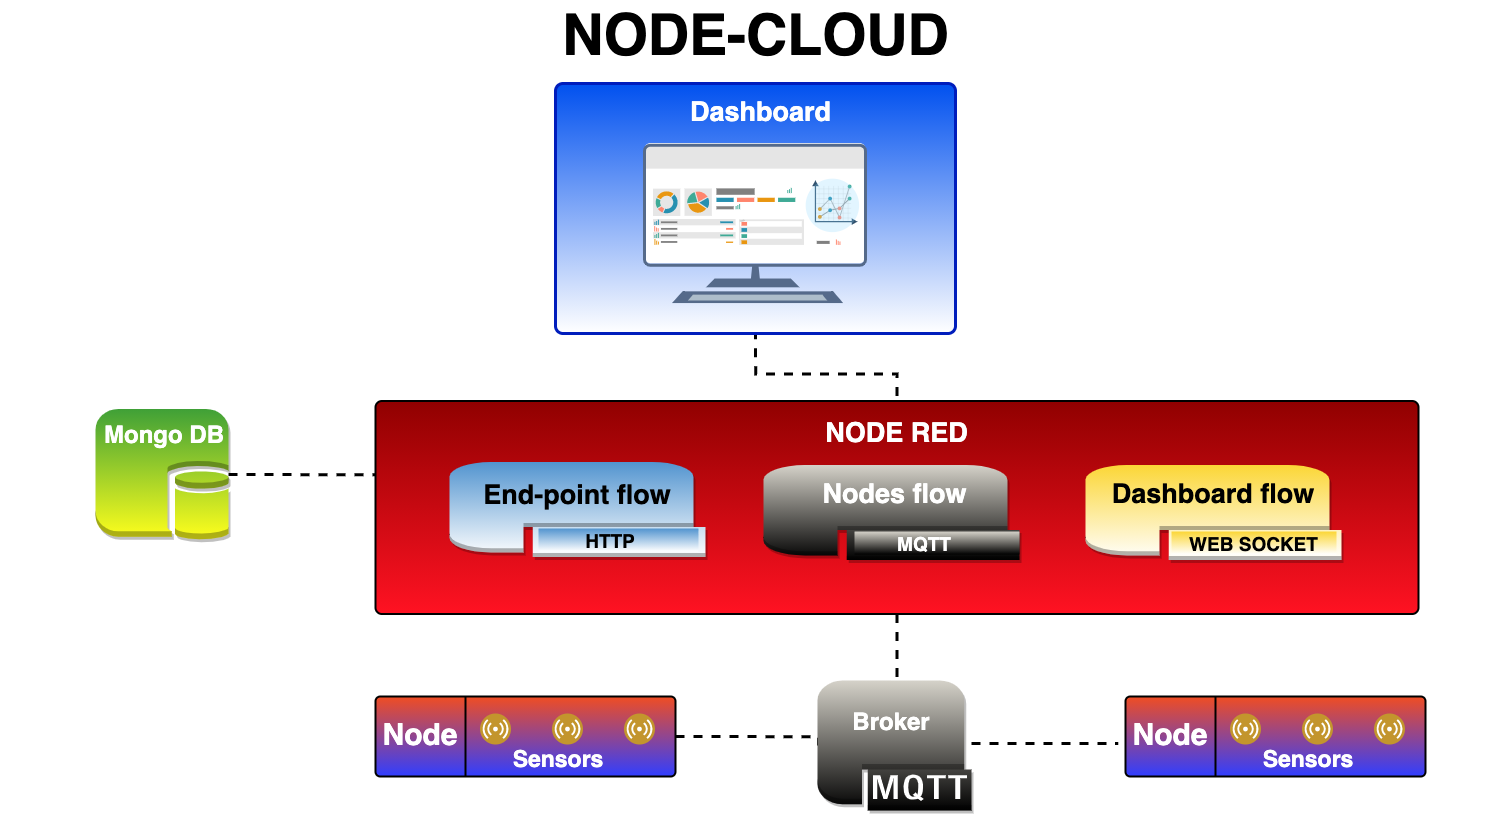
\includegraphics[width=0.9\textwidth]{Node Cloud Architecture.png}
    \caption{Architettura di Node-Cloud.}
    \label{fig:node-cloud-architecture}
\end{figure}
\subsection{Implementazione}
L’implementazione di Node-Cloud ha richiesto l’utilizzo di linguaggi e tecnologie differenti. In questa sezione saranno analizzate le specifiche componenti con riferimento alle librerie di supporto e alle modalità di comunicazione.
\paragraph{Core}
Il core del sistema, implementato con Node-RED, è costituito da tre flussi di base. I principali compiti sono:
\begin{itemize}
    \item costituire gli end-point \emph{HTTP}, grazie ai quali le componenti potranno richiedere le informazioni persistenti;
    \item recuperare i dati raccolti dai vari sensori, registrandosi agli appositi topic \emph{MQTT};
    \item gestire la comunicazione bidirezionale, real-time, implementata tramite \emph{WebSocket API}.
\end{itemize}
\paragraph{Database}
L’accesso alla base di dati è mediato da Node-RED, in modo tale da garantire un maggiore disaccoppiamento dalle varie componenti. La scelta è stata guidata dal desiderio di realizzare un sistema schemaless per la rappresentazione delle informazioni. Piuttosto che utilizzare un tradizionale data base \emph{SQL} è stata preferita l’adozione di \emph{MongoDB}\footnote{https://www.mongodb.com/}.

\paragraph{Sorgente Dati}
Affinché un sistema di monitoraggio possa svolgere il suo lavoro è indispensabile la presenza di una sorgente che fornisca i dati da analizzare. Nel caso di Node-Cloud è stato implementato un client Java, figura \ref{fig:java-client-architecture}, che simula il raccoglimento delle informazioni. Sensori di natura diversa campionano a intervalli regolari il contesto in cui sono immersi. Ogni sensore è eseguito su un apposito nodo di elaborazione. Per una gestione migliore dei vari nodi è stato introdotto un manager. I suoi compiti prevedono:
\begin{itemize}
    \item l’inizializzazione di nodi e sensori, recuperando le informazioni di configurazione necessarie tramite richieste HTTP;
    \item la pubblicazione dei dati raccolti dai sensori sull’apposito topic MQTT. Questa è la funzione fondamentale che consente di mettere in moto le elaborazioni del resto del sistema;
    \item la sottoscrizione al topic MQTT che consente di avviare i processi di attuazione. Tramite Node-Cloud possono essere modificate, in tempo reale, i parametri di configurazione di nodi e sensori. I comandi provenienti dalla GUI, una volta processati da Node-RED, saranno inoltrati al gestore al fine di controllare i dispositivi.
\end{itemize}
\begin{figure}[htb]
    \centering
    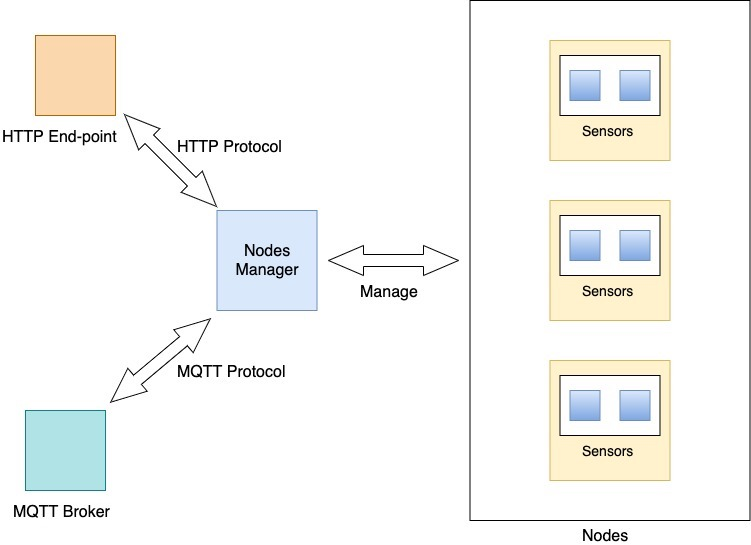
\includegraphics[width=0.80\textwidth]{java client.jpeg}
    \caption{Architettura del client Java.}
    \label{fig:java-client-architecture}
\end{figure}
L’utilizzo del protocollo MQTT richiede la presenza di un broker. Svariate sono le soluzioni disponibili, tra esse si è optato per quella fornita dall’ \emph{Eclipse Project}\footnote{https://mqtt.eclipseprojects.io/}.
\paragraph{Dashboard}
\emph{Node-Cloud} è stato progettato per essere una web application. In aggiunta alla componente server, realizzata con Node-RED, è stato implementato, seguendo un approccio single-page application (SPA), un web client.

La dashboard di Node-Cloud presenta una serie di indicatori che consentono di avere una panoramica generale sull’andamento dei nodi e dei sensori. In fase di caricamento vengono effettuate tre richieste asincrone di tipo HTTP agli end-point implementati con Node-RED. Sarà compito del server accedere alle collezioni del database restituendo al client, in formato JSON, le informazioni di configurazione. Il contenuto delle richieste verrà utilizzato per inizializzare indicatori e grafici. È importante sottolineare come, in linea con il modello SPA, le richieste esplicite avvengano solo in questa fase.

\subsection{Funzionalità}
Per poter identificare le funzionalità che un prodotto software dovrà esibire è molto importante calarsi nel contesto. Un sistema di monitoraggio, in primo luogo, deve consentire all’utente di visualizzare una serie di informazioni della realtà in esame. A tal fine, per il web client di Node-Cloud, sono state previste:
\begin{itemize}
    \item una dashboard, figura \ref{fig:node-cloud-dashboard}, grazie alla quale è possibile avere una visione d’insieme sul funzionamento dei dispositivi connessi. Oltre a poter visualizzare il numero totale di nodi e sensori e quanti di essi siano effettivamente disponibili, è riportato il numero di campioni rilevati. È possibile visualizzare quest’ultima informazione con diversi livelli di aggregazione:
    \begin{itemize}
        \item numero totale di campioni raccolti;
        \item numero di campioni raccolti per ogni nodo;
        \item numero di campioni raccolti da ogni singolo sensore.
    \end{itemize}
    In aggiunta è possibile modificare, in modo interattivo, il focus delle informazioni mostrate nei grafici.
    \item un’apposita sezione con la quale è possibile visualizzare i dettagli di ogni singolo sensore registrato, figura \ref{fig:sensor-page}. Tra cui:
    \begin{itemize}
        \item informazioni sul nodo di elaborazione sul quale sono istallati;
        \item specifiche tecniche;
        \item numero totale e media pesata dei campioni rilevati;
        \item time line in live-streaming per il monitoraggio dei dati prelevati. È possibile visualizzare lo storico dei campioni, modificare lo zoom e mettere in pausa/riprendere il flusso dei dati.
    \end{itemize}
\end{itemize}
\begin{figure}[H]
    \centering
    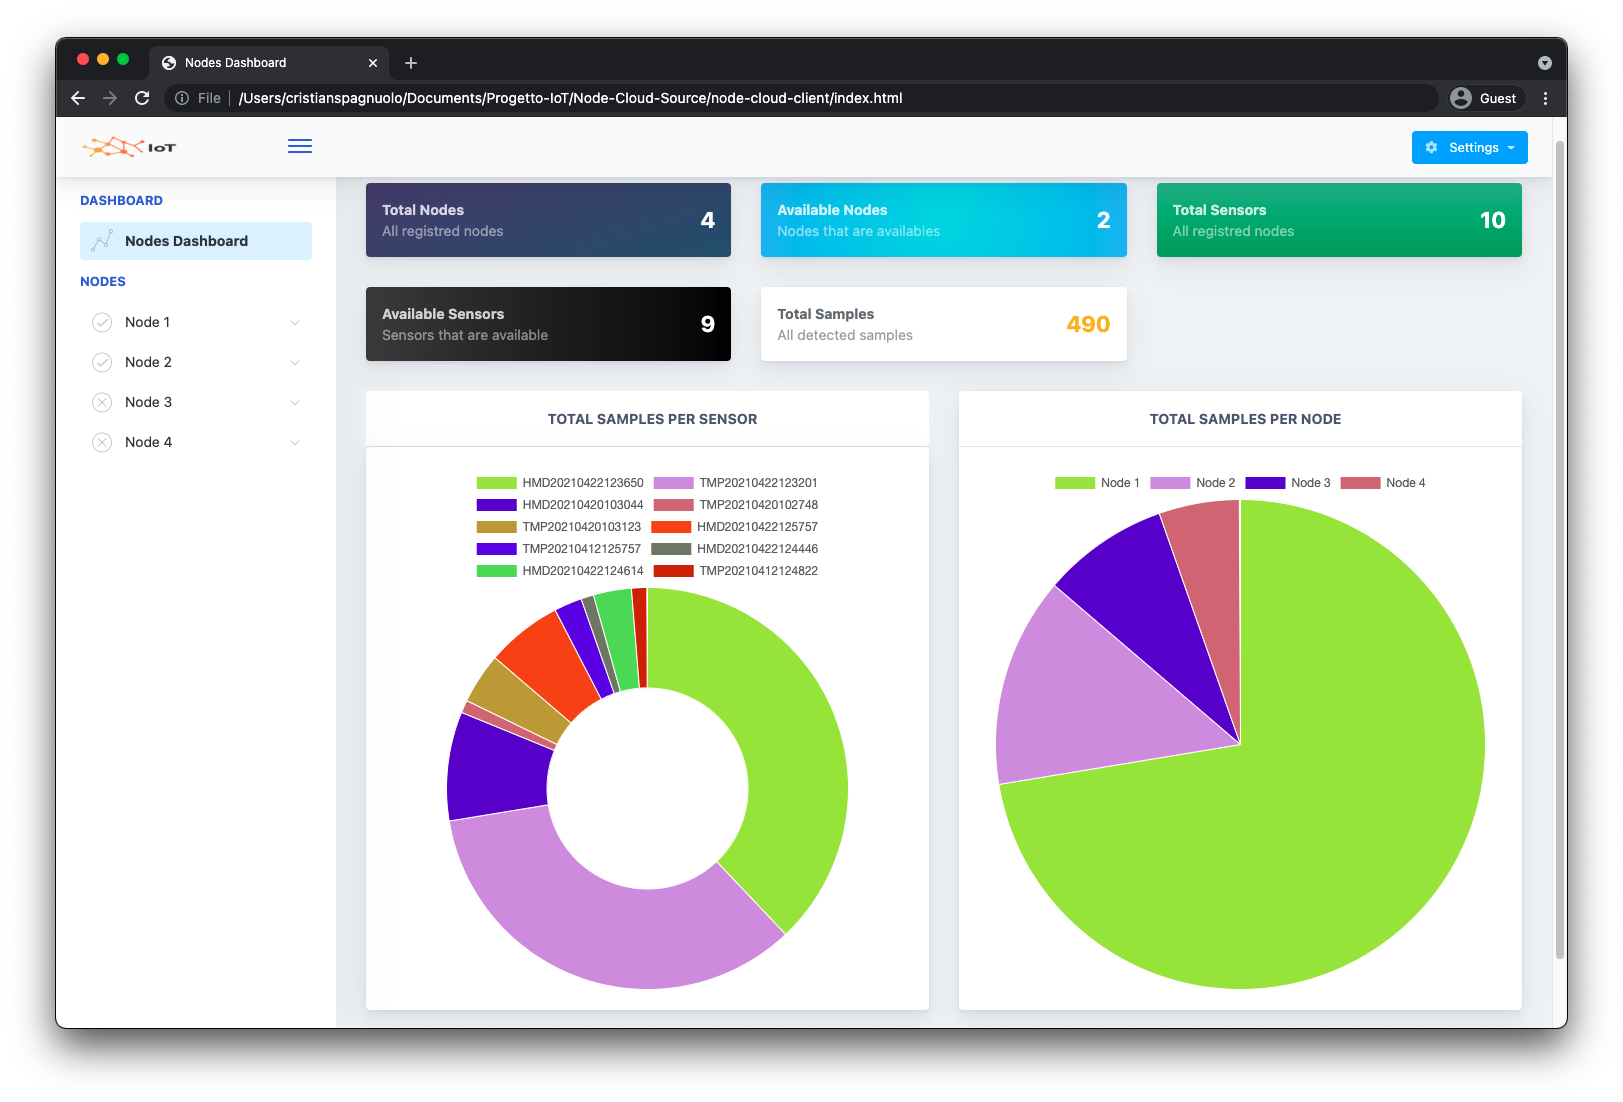
\includegraphics[width=0.80\textwidth]{dashboard.png}
    \caption{Dashboard di Node Cloud.}
    \label{fig:node-cloud-dashboard}
\end{figure}

\begin{figure}[H]
    \centering
     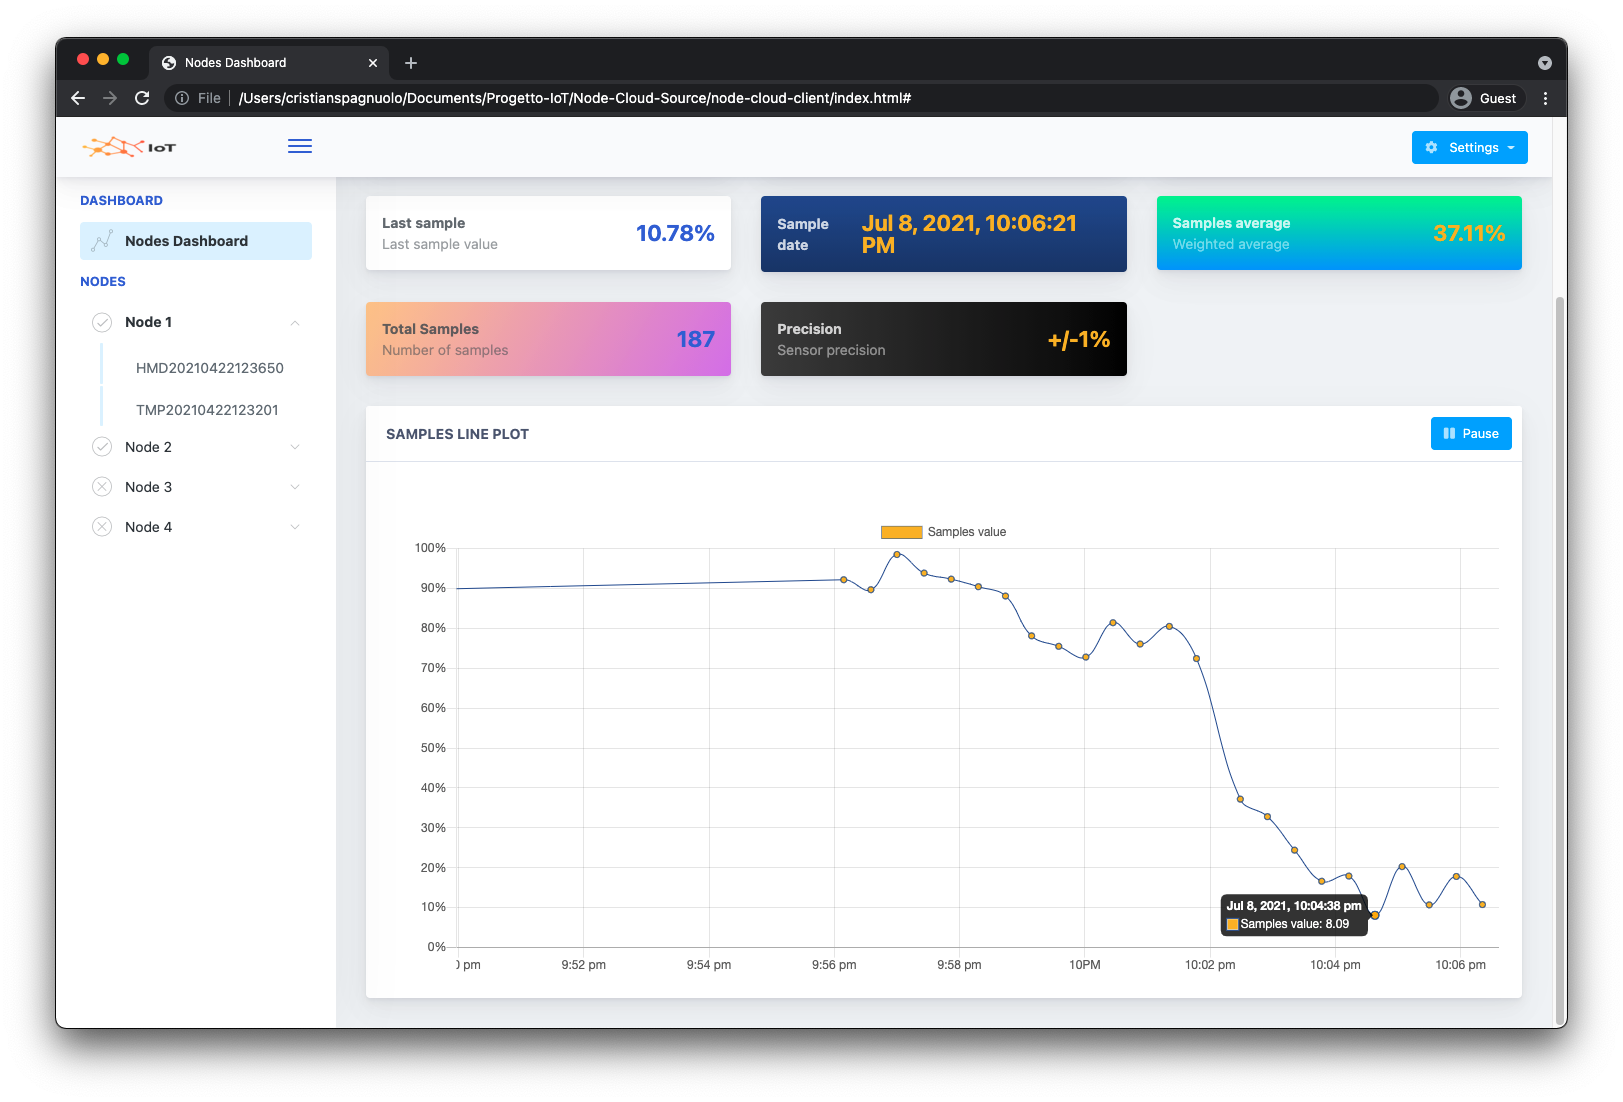
\includegraphics[width=0.80\textwidth]{sensor-page.png}
    \caption{Pagina del singolo sensor.}
    \label{fig:sensor-page}
\end{figure}
Il modello adottato per poter modificare i parametri di configurazione dei dispositivi è basato sulla modifica delle proprietà dell’entità stessa. A ogni comando è stato assegnato un topic differente, in fase di ricezione del messaggio verrà modificata l’opportuna proprietà per poi effettuare un riavvio del dispositivo.
La soluzione scelta introduce una serie di limiti. In primo luogo, individuiamo la necessità di dover utilizzare topic diversi, uno per ogni comando implementato. In secondo luogo, manca un’interfaccia comune per poter interagire in modo analogo con la grande vastità di dispositivi presenti sul mercato. Sviluppi futuri del sistema presentato si prefiggeranno l’obiettivo di far fronte a queste problematiche.
\emph{Node-Cloud} è in grado di pilotare i dispositivi connessi in tre diverse modalità:
\clearpage
\begin{itemize}
    \item è possibile attivare o disattivare un sensore, in tempo reale, premendo sul
widget della disponibilità.
\begin{figure}[H]
    \centering
     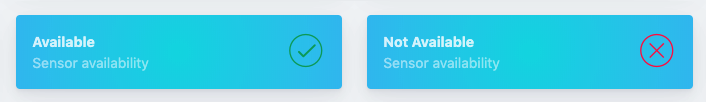
\includegraphics[width=0.80\textwidth]{change availability of sensor.png}
    \caption{Bottone per modificare la disponibilità del singolo sensore.}
    \label{fig:availability-button}
\end{figure}
\item tramite l’apposito pannello di amministrazione è possibile configurare i sensori, modificandone il tempo di campionamento, la disponibilità e la precisione;
\begin{figure}[H]
    \centering
     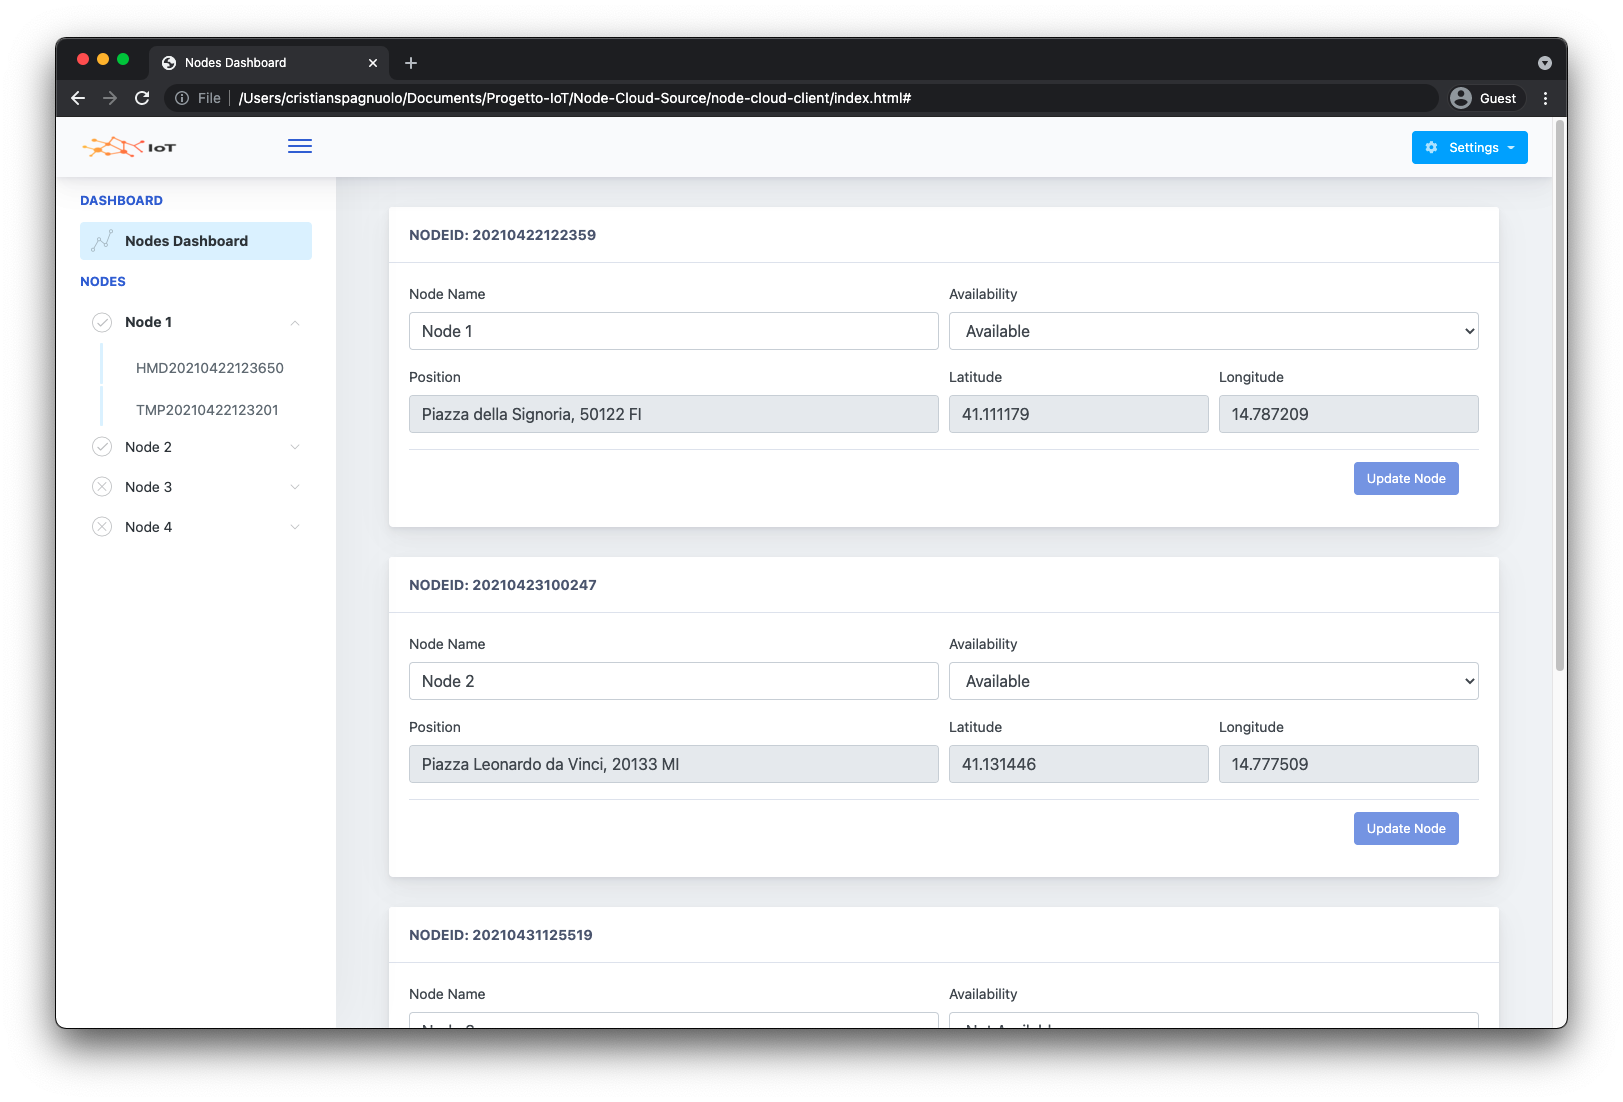
\includegraphics[width=0.80\textwidth]{nodes-management.png}
    \caption{Pannello di amministrazione dei nodi.}
    \label{fig:nodes-management}
\end{figure}
\item in modo analogo a quanto previsto per la gestione dei sensori, è stato realizzato un pannello di amministrazione anche per i nodi.
\begin{figure}[H]
    \centering
     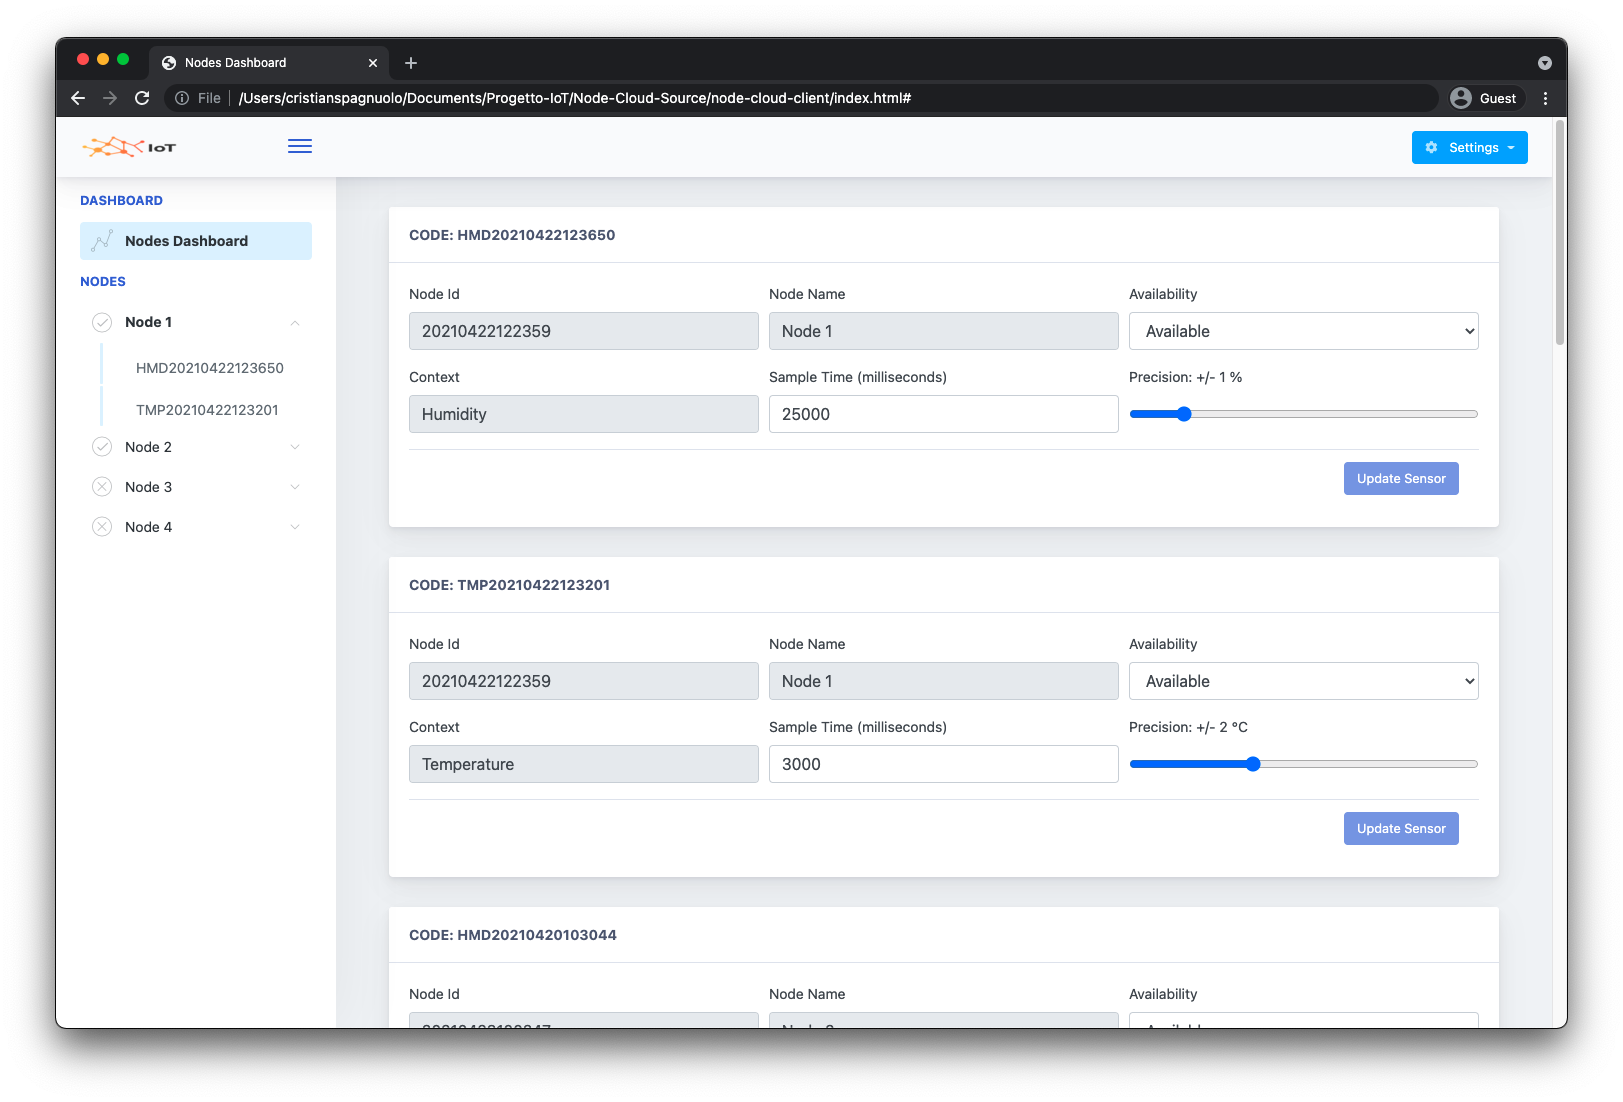
\includegraphics[width=0.80\textwidth]{sensors-management.png}
    \caption{Pannello di amministrazione dei sensori.}
    \label{fig:sensor-management}
\end{figure}
\end{itemize}
\section{Conclusioni}
Una delle principali caratteristiche dei dispositivi IoT è legata al grado di connessione con il contesto. Ogni sensore può essere considerato come una sorgente di informazioni, le quali dovranno essere processate dalle altre componenti applicative. L’enorme varietà di sensori disponibili sul mercato introduce problemi di eterogeneità dei dati raccolti.\newline

Node-Cloud è in grado di fornire una soluzione al problema, grazie a Node-RED, fungendo al contempo sia da gateway che da context broker. Il core offre la possibilità di modellare le informazioni di contesto al fine di disaccoppiare il formato originale dei dati da quello che sarà utilizzato per la comunicazione con le altre componenti. Nel caso in esame, la sorgente di campioni è stata simulata tramite un client Java. In futuro, per sostituire la sorgente con uno o più dispositivi fisici, sarà sufficiente introdurre degli appositi flussi che renderanno le nuove informazioni “consumabili” dalle altre componenti.\newline

Così come ogni altro prodotto software, anche Node-Cloud presenta una serie di limitazioni, le quali saranno affrontate in sviluppi futuri. In primo luogo, dovrà essere realizzata un’interfaccia che consenta di inserire un nuovo dispositivo, fisico o virtuale. Per farlo, è stata pensata l’implementazione di un apposito form, all’interno del web client, che consenta l’aggiunta dinamica di nuovi campi, ognuno dei quali in grado di supportare diversi tipi di dati. Inserite le informazioni, esse dovranno giungere al core del sistema, il quale avrà il compito di occuparsi dell’individuazione del dispositivo, nel caso in cui fosse fisico. Infine, un feedback sull’esito dell’operazione dovrà essere veicolato all’utente.\newline 

Un’altra funzionalità che potrebbe essere aggiunta in un secondo momento riguarda la possibilità di creare e gestire entità di contesto logiche sulla base di quelli che sono i nodi e i sensori registrati. A loro volta, anche le entità logiche potranno essere aggregate nuovamente tra loro. Ciò consentirebbe di migliorare la tolleranza ai guasti del sistema, mediante replicazione dei dispositivi, o ancora di sfruttare una serie di sensori di natura diversa, al fine di ottenere una grandezza composta come risultato delle misurazioni.
\end{document}